

\tikzset{every picture/.style={line width=0.75pt}} %set default line width to 0.75pt        

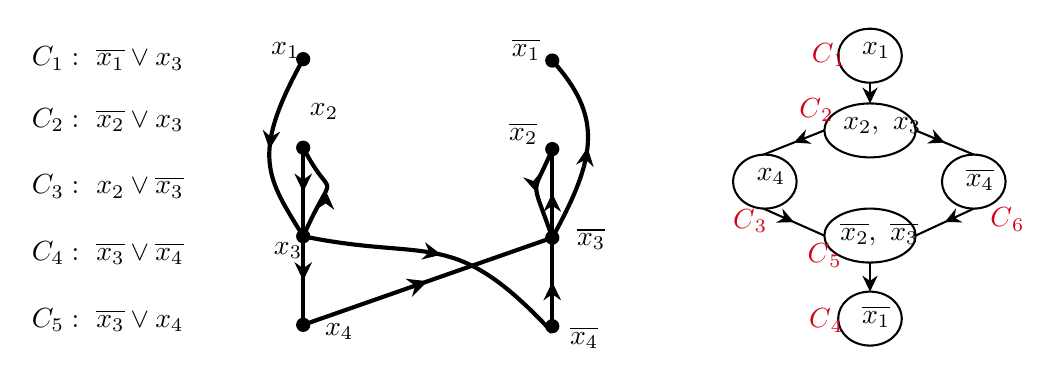
\begin{tikzpicture}[x=0.5pt,y=0.5pt,yscale=-1,xscale=1]
%uncomment if require: \path (0,257); %set diagram left start at 0, and has height of 257

%Flowchart: Connector [id:dp3724199168464428] 
\draw  [fill={rgb, 255:red, 0; green, 0; blue, 0 }  ,fill opacity=1 ] (206,32) .. controls (206,29.58) and (207.96,27.62) .. (210.38,27.62) .. controls (212.79,27.62) and (214.75,29.58) .. (214.75,32) .. controls (214.75,34.42) and (212.79,36.38) .. (210.38,36.38) .. controls (207.96,36.38) and (206,34.42) .. (206,32) -- cycle ;
%Straight Lines [id:da21698138157344438] 
\draw [color={rgb, 255:red, 0; green, 0; blue, 0 }  ,draw opacity=1 ][line width=1.5]    (210.38,224) -- (390.38,161.01) ;
\draw [shift={(300.38,192.5)}, rotate = 520.71] [fill={rgb, 255:red, 0; green, 0; blue, 0 }  ,fill opacity=1 ][line width=0.08]  [draw opacity=0] (14.56,-6.99) -- (0,0) -- (14.56,6.99) -- (9.67,0) -- cycle    ;
%Flowchart: Connector [id:dp10381668129107124] 
\draw  [fill={rgb, 255:red, 0; green, 0; blue, 0 }  ,fill opacity=1 ] (206,96) .. controls (206,93.59) and (207.96,91.63) .. (210.38,91.63) .. controls (212.79,91.63) and (214.75,93.59) .. (214.75,96) .. controls (214.75,98.42) and (212.79,100.38) .. (210.38,100.38) .. controls (207.96,100.38) and (206,98.42) .. (206,96) -- cycle ;
%Flowchart: Connector [id:dp3907425587900879] 
\draw  [fill={rgb, 255:red, 0; green, 0; blue, 0 }  ,fill opacity=1 ] (206,160.01) .. controls (206,157.59) and (207.96,155.63) .. (210.38,155.63) .. controls (212.79,155.63) and (214.75,157.59) .. (214.75,160.01) .. controls (214.75,162.42) and (212.79,164.38) .. (210.38,164.38) .. controls (207.96,164.38) and (206,162.42) .. (206,160.01) -- cycle ;
%Flowchart: Connector [id:dp7417499401424387] 
\draw  [fill={rgb, 255:red, 0; green, 0; blue, 0 }  ,fill opacity=1 ] (206,224) .. controls (206,221.58) and (207.96,219.62) .. (210.38,219.62) .. controls (212.79,219.62) and (214.75,221.58) .. (214.75,224) .. controls (214.75,226.42) and (212.79,228.38) .. (210.38,228.38) .. controls (207.96,228.38) and (206,226.42) .. (206,224) -- cycle ;
%Flowchart: Connector [id:dp6925277380251512] 
\draw  [fill={rgb, 255:red, 0; green, 0; blue, 0 }  ,fill opacity=1 ] (386,33) .. controls (386,30.58) and (387.96,28.62) .. (390.38,28.62) .. controls (392.79,28.62) and (394.75,30.58) .. (394.75,33) .. controls (394.75,35.42) and (392.79,37.38) .. (390.38,37.38) .. controls (387.96,37.38) and (386,35.42) .. (386,33) -- cycle ;
%Flowchart: Connector [id:dp39532236220272543] 
\draw  [fill={rgb, 255:red, 0; green, 0; blue, 0 }  ,fill opacity=1 ] (386,97) .. controls (386,94.59) and (387.96,92.63) .. (390.38,92.63) .. controls (392.79,92.63) and (394.75,94.59) .. (394.75,97) .. controls (394.75,99.42) and (392.79,101.38) .. (390.38,101.38) .. controls (387.96,101.38) and (386,99.42) .. (386,97) -- cycle ;
%Flowchart: Connector [id:dp9098235514745779] 
\draw  [fill={rgb, 255:red, 0; green, 0; blue, 0 }  ,fill opacity=1 ] (386,161.01) .. controls (386,158.59) and (387.96,156.63) .. (390.38,156.63) .. controls (392.79,156.63) and (394.75,158.59) .. (394.75,161.01) .. controls (394.75,163.42) and (392.79,165.38) .. (390.38,165.38) .. controls (387.96,165.38) and (386,163.42) .. (386,161.01) -- cycle ;
%Flowchart: Connector [id:dp21395664195538067] 
\draw  [fill={rgb, 255:red, 0; green, 0; blue, 0 }  ,fill opacity=1 ] (386,225) .. controls (386,222.58) and (387.96,220.62) .. (390.38,220.62) .. controls (392.79,220.62) and (394.75,222.58) .. (394.75,225) .. controls (394.75,227.42) and (392.79,229.38) .. (390.38,229.38) .. controls (387.96,229.38) and (386,227.42) .. (386,225) -- cycle ;
%Straight Lines [id:da5808140188000758] 
\draw [line width=1.5]    (210.38,160.01) -- (210.38,96) ;
\draw [shift={(210.38,128)}, rotate = 270] [fill={rgb, 255:red, 0; green, 0; blue, 0 }  ][line width=0.08]  [draw opacity=0] (13.4,-6.43) -- (0,0) -- (13.4,6.44) -- (8.9,0) -- cycle    ;
%Curve Lines [id:da1567657256671482] 
\draw [line width=1.5]    (210.38,160.01) .. controls (302.5,179) and (318.5,152) .. (390.38,229.38) ;
\draw [shift={(310.17,173.29)}, rotate = 191.87] [fill={rgb, 255:red, 0; green, 0; blue, 0 }  ][line width=0.08]  [draw opacity=0] (13.4,-6.43) -- (0,0) -- (13.4,6.44) -- (8.9,0) -- cycle    ;
%Curve Lines [id:da2728531907004703] 
\draw [line width=1.5]    (210.38,96) .. controls (232.5,139) and (234.5,106) .. (210.38,160.01) ;
\draw [shift={(226.81,127.36)}, rotate = 91.46] [fill={rgb, 255:red, 0; green, 0; blue, 0 }  ][line width=0.08]  [draw opacity=0] (13.4,-6.43) -- (0,0) -- (13.4,6.44) -- (8.9,0) -- cycle    ;
%Curve Lines [id:da6712774074376199] 
\draw [line width=1.5]    (390.38,161.01) .. controls (374.5,115.01) and (375.5,133) .. (390.38,97) ;
\draw [shift={(379.15,128.57)}, rotate = 254.32] [fill={rgb, 255:red, 0; green, 0; blue, 0 }  ][line width=0.08]  [draw opacity=0] (13.4,-6.43) -- (0,0) -- (13.4,6.44) -- (8.9,0) -- cycle    ;
%Curve Lines [id:da0994531296434309] 
\draw [line width=1.5]    (210.38,32) .. controls (171.5,102) and (184.5,118) .. (210.38,160.01) ;
\draw [shift={(185.99,96.97)}, rotate = 276.2] [fill={rgb, 255:red, 0; green, 0; blue, 0 }  ][line width=0.08]  [draw opacity=0] (13.4,-6.43) -- (0,0) -- (13.4,6.44) -- (8.9,0) -- cycle    ;
%Curve Lines [id:da4618567980931958] 
\draw [line width=1.5]    (390.38,161.01) .. controls (423.12,102) and (426.5,73) .. (390.38,33) ;
\draw [shift={(415.82,95.84)}, rotate = 458.06] [fill={rgb, 255:red, 0; green, 0; blue, 0 }  ][line width=0.08]  [draw opacity=0] (13.4,-6.43) -- (0,0) -- (13.4,6.44) -- (8.9,0) -- cycle    ;
%Straight Lines [id:da681306498318515] 
\draw [line width=1.5]    (390.38,97) -- (390.38,161.01) ;
\draw [shift={(390.38,129)}, rotate = 90] [fill={rgb, 255:red, 0; green, 0; blue, 0 }  ][line width=0.08]  [draw opacity=0] (13.4,-6.43) -- (0,0) -- (13.4,6.44) -- (8.9,0) -- cycle    ;
%Straight Lines [id:da7450683269718487] 
\draw [line width=1.5]    (210.38,224) -- (210.38,160.01) ;
\draw [shift={(210.38,192)}, rotate = 270] [fill={rgb, 255:red, 0; green, 0; blue, 0 }  ][line width=0.08]  [draw opacity=0] (13.4,-6.43) -- (0,0) -- (13.4,6.44) -- (8.9,0) -- cycle    ;
%Straight Lines [id:da28446201940975424] 
\draw [line width=1.5]    (390.38,161.01) -- (390.38,225) ;
\draw [shift={(390.38,193)}, rotate = 90] [fill={rgb, 255:red, 0; green, 0; blue, 0 }  ][line width=0.08]  [draw opacity=0] (13.4,-6.43) -- (0,0) -- (13.4,6.44) -- (8.9,0) -- cycle    ;
%Straight Lines [id:da8993012890613198] 
\draw [color={rgb, 255:red, 0; green, 0; blue, 0 }  ,draw opacity=1 ][line width=0.75]    (543,101) -- (587,83.5) ;
\draw [shift={(565,92.25)}, rotate = 338.31] [fill={rgb, 255:red, 0; green, 0; blue, 0 }  ,fill opacity=1 ][line width=0.08]  [draw opacity=0] (11.61,-5.58) -- (0,0) -- (11.61,5.58) -- (7.71,0) -- cycle    ;
%Shape: Ellipse [id:dp4222608559717377] 
\draw   (597,29.5) .. controls (597,18.73) and (607.3,10) .. (620,10) .. controls (632.7,10) and (643,18.73) .. (643,29.5) .. controls (643,40.27) and (632.7,49) .. (620,49) .. controls (607.3,49) and (597,40.27) .. (597,29.5) -- cycle ;

%Shape: Ellipse [id:dp48489763152887844] 
\draw   (587,83.5) .. controls (587,72.73) and (601.77,64) .. (620,64) .. controls (638.23,64) and (653,72.73) .. (653,83.5) .. controls (653,94.27) and (638.23,103) .. (620,103) .. controls (601.77,103) and (587,94.27) .. (587,83.5) -- cycle ;

%Shape: Ellipse [id:dp23487748011023923] 
\draw   (587,159.5) .. controls (587,148.73) and (601.77,140) .. (620,140) .. controls (638.23,140) and (653,148.73) .. (653,159.5) .. controls (653,170.27) and (638.23,179) .. (620,179) .. controls (601.77,179) and (587,170.27) .. (587,159.5) -- cycle ;
%Shape: Ellipse [id:dp8959213833983161] 
\draw   (521,120.5) .. controls (521,109.73) and (531.3,101) .. (544,101) .. controls (556.7,101) and (567,109.73) .. (567,120.5) .. controls (567,131.27) and (556.7,140) .. (544,140) .. controls (531.3,140) and (521,131.27) .. (521,120.5) -- cycle ;
%Shape: Ellipse [id:dp5504797296350772] 
\draw   (672,120.5) .. controls (672,109.73) and (682.3,101) .. (695,101) .. controls (707.7,101) and (718,109.73) .. (718,120.5) .. controls (718,131.27) and (707.7,140) .. (695,140) .. controls (682.3,140) and (672,131.27) .. (672,120.5) -- cycle ;
%Shape: Ellipse [id:dp9111616138087153] 
\draw   (597,219.5) .. controls (597,208.73) and (607.3,200) .. (620,200) .. controls (632.7,200) and (643,208.73) .. (643,219.5) .. controls (643,230.27) and (632.7,239) .. (620,239) .. controls (607.3,239) and (597,230.27) .. (597,219.5) -- cycle ;
%Straight Lines [id:da20036758362743068] 
\draw [color={rgb, 255:red, 0; green, 0; blue, 0 }  ,draw opacity=1 ][line width=0.75]    (620,61) -- (620,49) ;
\draw [shift={(620,64)}, rotate = 270] [fill={rgb, 255:red, 0; green, 0; blue, 0 }  ,fill opacity=1 ][line width=0.08]  [draw opacity=0] (11.61,-5.58) -- (0,0) -- (11.61,5.58) -- (7.71,0) -- cycle    ;
%Straight Lines [id:da09641247447116963] 
\draw [color={rgb, 255:red, 0; green, 0; blue, 0 }  ,draw opacity=1 ][line width=0.75]    (695,101) -- (653,83.5) ;
\draw [shift={(674,92.25)}, rotate = 202.62] [fill={rgb, 255:red, 0; green, 0; blue, 0 }  ,fill opacity=1 ][line width=0.08]  [draw opacity=0] (11.61,-5.58) -- (0,0) -- (11.61,5.58) -- (7.71,0) -- cycle    ;
%Straight Lines [id:da875967903250598] 
\draw [color={rgb, 255:red, 0; green, 0; blue, 0 }  ,draw opacity=1 ][line width=0.75]    (653,159.5) -- (695,140) ;
\draw [shift={(674,149.75)}, rotate = 335.1] [fill={rgb, 255:red, 0; green, 0; blue, 0 }  ,fill opacity=1 ][line width=0.08]  [draw opacity=0] (11.61,-5.58) -- (0,0) -- (11.61,5.58) -- (7.71,0) -- cycle    ;
%Straight Lines [id:da19792854880744393] 
\draw [color={rgb, 255:red, 0; green, 0; blue, 0 }  ,draw opacity=1 ][line width=0.75]    (587,159.5) -- (543,140) ;
\draw [shift={(565,149.75)}, rotate = 203.9] [fill={rgb, 255:red, 0; green, 0; blue, 0 }  ,fill opacity=1 ][line width=0.08]  [draw opacity=0] (11.61,-5.58) -- (0,0) -- (11.61,5.58) -- (7.71,0) -- cycle    ;
%Straight Lines [id:da23800394462691676] 
\draw [color={rgb, 255:red, 0; green, 0; blue, 0 }  ,draw opacity=1 ][line width=0.75]    (620,197) -- (620,179) ;
\draw [shift={(620,200)}, rotate = 270] [fill={rgb, 255:red, 0; green, 0; blue, 0 }  ,fill opacity=1 ][line width=0.08]  [draw opacity=0] (11.61,-5.58) -- (0,0) -- (11.61,5.58) -- (7.71,0) -- cycle    ;

% Text Node
\draw (12,21) node [anchor=north west][inner sep=0.75pt]   [align=left] {$\displaystyle C_{1} :\ \overline{x_{1}} \lor x_{3}$};
% Text Node
\draw (12,65.25) node [anchor=north west][inner sep=0.75pt]   [align=left] {$\displaystyle C_{2} :\ \overline{x_{2}} \lor x_{3}$};
% Text Node
\draw (12,113.5) node [anchor=north west][inner sep=0.75pt]   [align=left] {$\displaystyle C_{3} :\ x_{2} \lor \overline{x_{3}}$};
% Text Node
\draw (12,161.75) node [anchor=north west][inner sep=0.75pt]   [align=left] {$\displaystyle C_{4} :\ \overline{x_{3}} \lor \overline{x_{4}}$};
% Text Node
\draw (12,210) node [anchor=north west][inner sep=0.75pt]   [align=left] {$\displaystyle C_{5} :\ \overline{x_{3}} \lor x_{4}$};
% Text Node
\draw (185,18) node [anchor=north west][inner sep=0.75pt]   [align=left] {$\displaystyle x_{1}$};
% Text Node
\draw (213,62) node [anchor=north west][inner sep=0.75pt]   [align=left] {$\displaystyle x_{2}$};
% Text Node
\draw (187,162) node [anchor=north west][inner sep=0.75pt]   [align=left] {$\displaystyle x_{3}$};
% Text Node
\draw (224,221) node [anchor=north west][inner sep=0.75pt]   [align=left] {$\displaystyle x_{4}$};
% Text Node
\draw (359,15) node [anchor=north west][inner sep=0.75pt]   [align=left] {$\displaystyle \overline{x_{1}}$};
% Text Node
\draw (357,76) node [anchor=north west][inner sep=0.75pt]   [align=left] {$\displaystyle \overline{x_{2}}$};
% Text Node
\draw (406,152) node [anchor=north west][inner sep=0.75pt]   [align=left] {$\displaystyle \overline{x_{3}}$};
% Text Node
\draw (401,223) node [anchor=north west][inner sep=0.75pt]   [align=left] {$\displaystyle \overline{x_{4}}$};
% Text Node
\draw (575.75,18.35) node [anchor=north west][inner sep=0.75pt]   [align=left] {$\displaystyle \textcolor[rgb]{0.82,0.01,0.11}{C}\textcolor[rgb]{0.82,0.01,0.11}{_{1}}$};
% Text Node
\draw (612,18) node [anchor=north west][inner sep=0.75pt]   [align=left] {$\displaystyle x_{1}$};
% Text Node
\draw (598.43,72) node [anchor=north west][inner sep=0.75pt]   [align=left] {$\displaystyle x_{2} ,\ x_{3}$};
% Text Node
\draw (596.43,148) node [anchor=north west][inner sep=0.75pt]   [align=left] {$\displaystyle \overline{x_{2}} ,\ \overline{x_{3}}$};
% Text Node
\draw (536,109) node [anchor=north west][inner sep=0.75pt]   [align=left] {$\displaystyle x_{4}$};
% Text Node
\draw (687,109) node [anchor=north west][inner sep=0.75pt]   [align=left] {$\displaystyle \overline{x_{4}}$};
% Text Node
\draw (612,208) node [anchor=north west][inner sep=0.75pt]   [align=left] {$\displaystyle \overline{x_{1}}$};
% Text Node
\draw (566.75,58.35) node [anchor=north west][inner sep=0.75pt]   [align=left] {$\displaystyle \textcolor[rgb]{0.82,0.01,0.11}{C}\textcolor[rgb]{0.82,0.01,0.11}{_{2}}$};
% Text Node
\draw (518.75,138.35) node [anchor=north west][inner sep=0.75pt]   [align=left] {$\displaystyle \textcolor[rgb]{0.82,0.01,0.11}{C}\textcolor[rgb]{0.82,0.01,0.11}{_{3}}$};
% Text Node
\draw (573.75,210.35) node [anchor=north west][inner sep=0.75pt]   [align=left] {$\displaystyle \textcolor[rgb]{0.82,0.01,0.11}{C}\textcolor[rgb]{0.82,0.01,0.11}{_{4}}$};
% Text Node
\draw (572.75,163.35) node [anchor=north west][inner sep=0.75pt]   [align=left] {$\displaystyle \textcolor[rgb]{0.82,0.01,0.11}{C}\textcolor[rgb]{0.82,0.01,0.11}{_{5}}$};
% Text Node
\draw (704.75,137.35) node [anchor=north west][inner sep=0.75pt]   [align=left] {$\displaystyle \textcolor[rgb]{0.82,0.01,0.11}{C}\textcolor[rgb]{0.82,0.01,0.11}{_{6}}$};


\end{tikzpicture}

